\documentclass[12pt]{article}
\usepackage[utf8]{inputenc}
\usepackage[english]{babel}
\usepackage{longtable}
\usepackage[hyphens,spaces,obeyspaces]{url}

\usepackage{amsmath,amsthm,amssymb,amsfonts}
\usepackage{booktabs}
\usepackage{array}
\usepackage{fancyhdr}
\usepackage[a4paper, margin=1in]{geometry}
\usepackage{enumerate}
\usepackage{graphicx}
\usepackage{subcaption}
\usepackage{hyperref}
\graphicspath{ {./images/} }

\newcommand{\N}{\mathbb{N}}
\newcommand{\Z}{\mathbb{Z}}
\newcommand{\R}{\mathbb{R}}
\newcommand{\mat}[1]{\mathbf{#1}}
\newcommand{\norm}[1]{\left\lVert#1\right\rVert}
\newcommand{\PreserveBackslash}[1]{\let\temp=\\#1\let\\=\temp}
\newcolumntype{C}[1]{>{\PreserveBackslash\centering}p{#1}}
\newcolumntype{R}[1]{>{\PreserveBackslash\raggedleft}p{#1}}
\newcolumntype{L}[1]{>{\PreserveBackslash\raggedright}p{#1}}

\pagestyle{fancy}
\fancyhf{}
\rhead{TSE, Ho Nam}
\chead{Project \#3}
\lhead{MATH4828B}
\cfoot{\thepage}
\title{
  {\large MATH4828B Machine Learning for Natural Language Processing}\\
  \textbf{\large Project 3 -- Language Model}\\
  \textbf{Report}
  }
\author{ 
  \begin{tabular}{R{0.4\textwidth}L{0.4\textwidth}}
    \textbf{Name:} & TSE, Ho Nam \\
    \textbf{Student ID:} & 20423612 \\
    \textbf{Dev Set Score:} & 1.3916
  \end{tabular}
 }
  
\date{}

\begin{document}
\maketitle\thispagestyle{fancy}
\tableofcontents
\section{Architectures}
There are two main types of architecture that I tried, and they are (i) LSTM and (ii) TCN.

\subsection{LSTM}
Long Short Term Memory (LSTM) is a type of Recurrent Neural Network (RNN) that aims to solve the problem of gradient explosion and diminishing problems in simple RNN. Comparing with simple RNN, LSTM can be trained using a longer sequence and usually performs better. In a LSTM cell (Figure~\ref{fig:LSTM}), there are four gates \(i, f, o, g\) and two hidden states \(c_t, h_t\). The equations for forward pass is as follows, with \(\odot\) being the elementwise multiplication, \(\sigma\) being the sigmoid activation and \(\tanh\) being the \(\tanh\) activation.
\[
	\begin{bmatrix}
		i \\ f \\ o \\ g
	\end{bmatrix}
	=
	\begin{bmatrix}
		\sigma \\ \sigma \\ \sigma \\ \tanh
	\end{bmatrix}
	\mat W
	\begin{bmatrix}
		\mat h_{t-1} \\ \mat x_t
	\end{bmatrix}
	,\qquad
	c_t = f \odot c_{t-1} + i \odot g
	,\qquad
	h_t = o \odot \tanh(c_t)
\]
The intuitive idea behind these equations is that, \(i\) governs how much information of \(x_t\) should be written to \(c_t\) and \(f\) governs how much information of \(c_{t-1}\) should be forgotten. \(g\) governs how much \(x_t\) is reach revealed to \(c_t\) and \(o\) governs how much \(c_t\) is written to \(h_t\). This new model works better than simple RNN because of the gradient highway along the \(c_t\) line which help solves the problem of gradient issues.

\begin{figure}[h!]
	\centering
	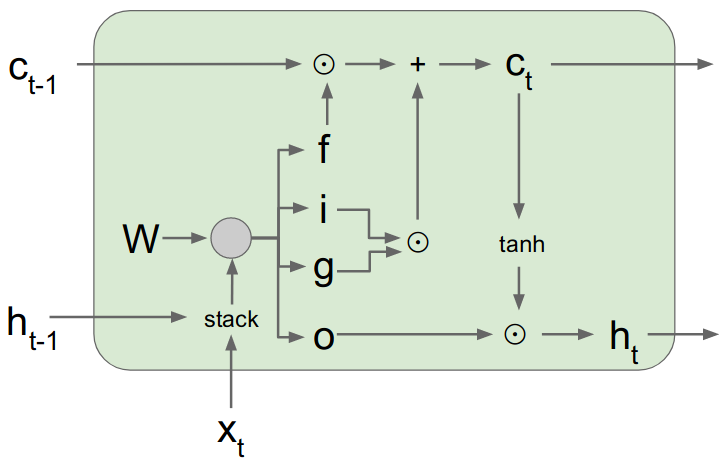
\includegraphics[width=0.5\linewidth]{LSTM}
	\caption{A LSTM cell.\protect\footnotemark}
	\label{fig:LSTM}
\end{figure}
\footnotetext{From Stanford cs231n lecture notes.}

Even LSTM is a better choice than simple RNN, it has a lot more parameters than simple RNN and generally it takes longer to train these models. Therefore, another alternative is explored for this project.
\subsection{TCN}
Temporal Convolutional Network (TCN) is a novel Convolutional Neural Network (CNN) modified to work on temporal domain introduced in early 2018. It uses a sequence of dilated convolutional layers, normalization layers, dropout layers and ReLU activations. From the authors\footnote{Bai, Shaojie, J. Zico Kolter, and Vladlen Koltun.``An empirical evaluation of generic convolutional and recurrent networks for sequence modeling.'' arXiv preprint arXiv:1803.01271 (2018).} of TCN, their experimental results show TCN outperforms simple RNN, LSTM and GRU in different sequence modelling tasks significantly. It can also exhibit a longer memory, and has stable gradients.

\begin{figure}[h!]
	\centering
	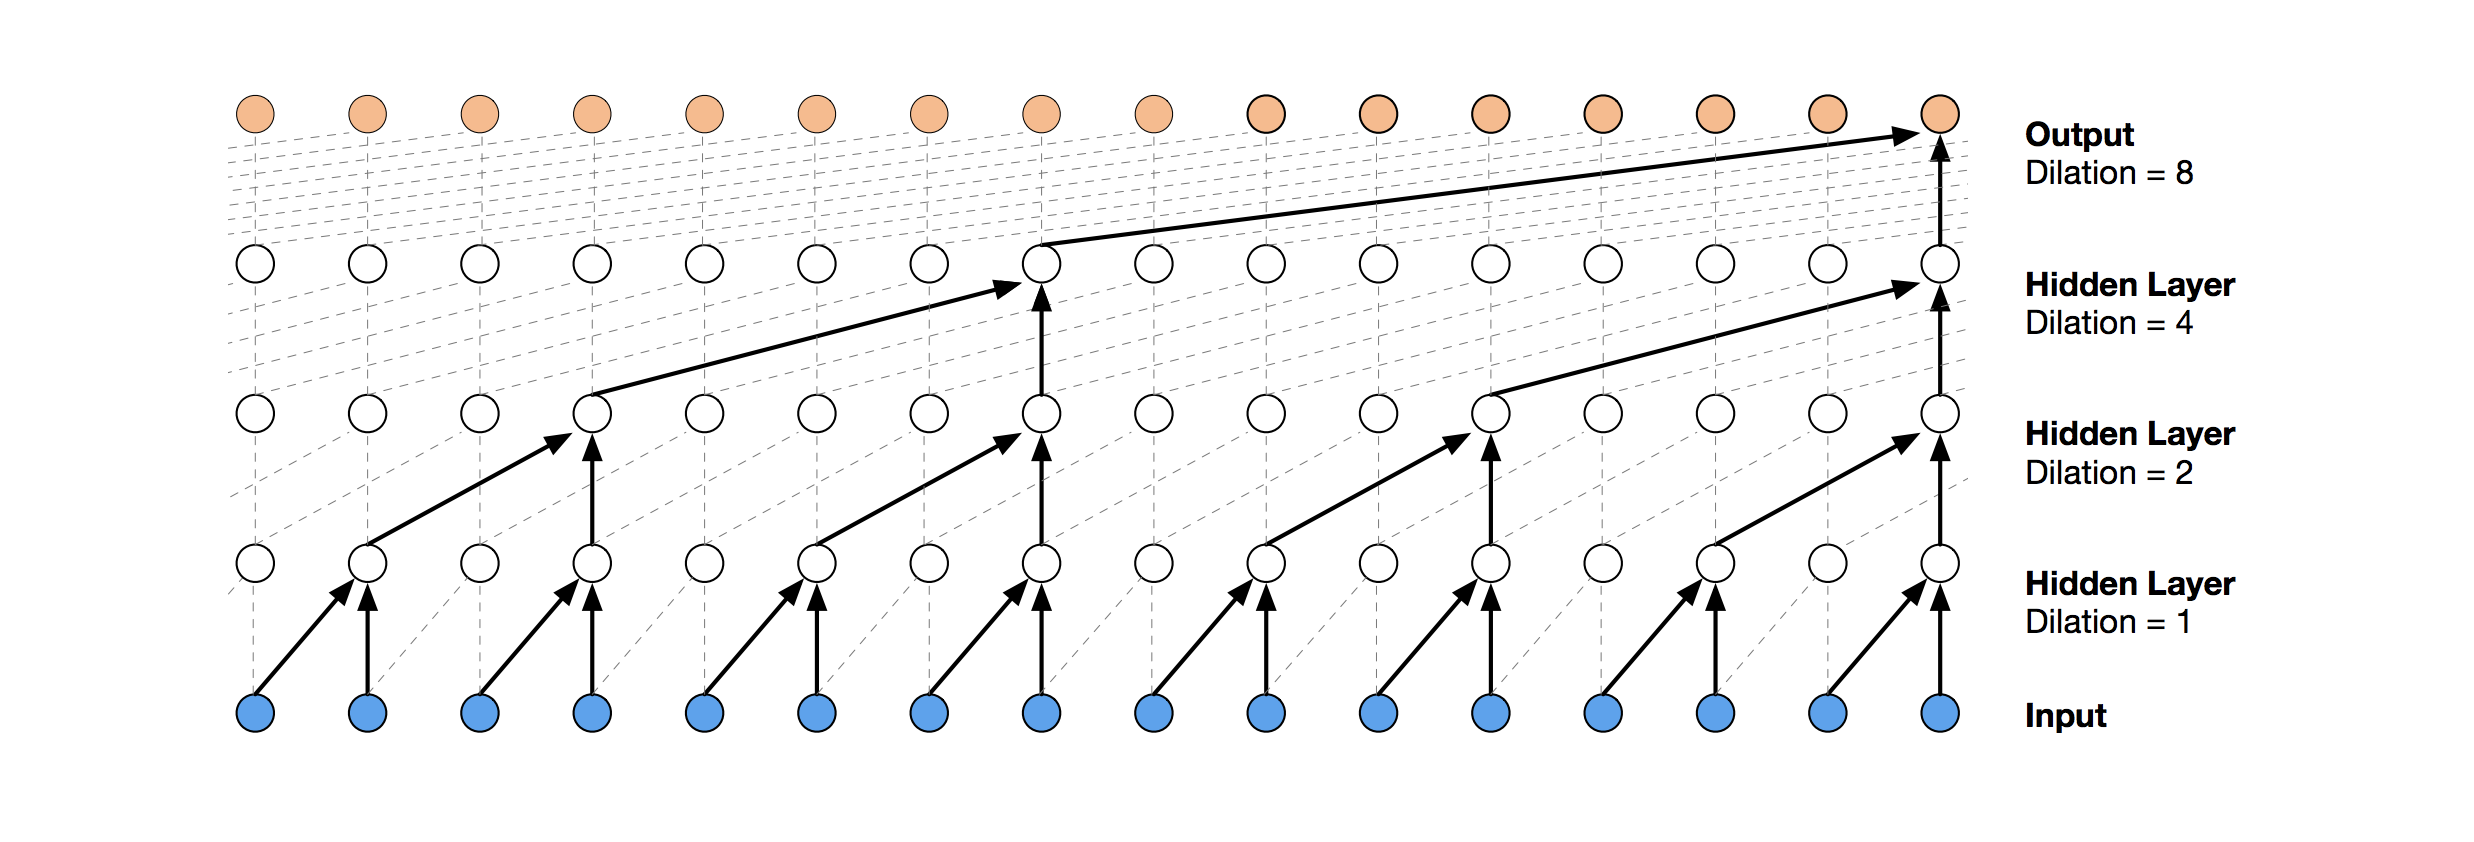
\includegraphics[width=\linewidth]{TCN}
	\caption{TCN strcuture.\protect\footnotemark}
	\label{fig:TCN}
\end{figure}
\footnotetext{From \url{https://github.com/philipperemy/keras-tcn}.}

\section{Experiments}
There were two phases of experiments. During the first phase, I used the provided sample code for generating training and validation data; while in the second phase, I reprogrammed these parts. There were in total around 200 sets of training records.

\subsection{Training with Provided Code}
There were multiple types of architectures attempted during this phase. They are constructed by LSTM, and/or TCN layers mentioned in the previous section. All models have a Embedding layer with various intermediate layer(s), then is finally fed into a Dense layer with softmax activation. The models include:

\begin{table}[h!]
	\centering
	\begin{tabular}{C{0.25\textwidth}C{0.65\textwidth}}
		\toprule
		Model Type                    & Architecture                                                      \\\midrule
		\texttt{lstm}                 & Embedding \(\to\) LSTM1 \(\to\) Dense                             \\\midrule
		\texttt{lstm2}                & Embedding \(\to\) LSTM1 \(\to\) LSTM2 \(\to\) Dense               \\\midrule
		\texttt{lstm3}                & Embedding \(\to\) LSTM1 \(\to\) LSTM2 \(\to\) LSTM3 \(\to\) Dense \\\midrule
		\texttt{lstm\_embed}          & Embedding \(\to\) LSTM1                                           \\
		                              & LSTM1 + Embedding \(\to\) Dense                                   \\\midrule
		\texttt{tcn}                  & Embedding \(\to\) TCN1 \(\to\) Dense                              \\\midrule
		\texttt{tcn\_embed}           & Embedding \(\to\) TCN1                                            \\
		                              & TCN1 + Embedding \(\to\) Dense                                    \\\midrule
		\texttt{tcn\_lstm}            & Embedding \(\to\) LSTM1                                           \\ & Embedding \(\to\) TCN1 \\ & TCN1 + LSTM1 \(\to\) Dense                                   \\\midrule
		\texttt{tcn\_lstm\_embed}     & Embedding \(\to\) LSTM1                                           \\ & Embedding \(\to\) TCN1 \\ & TCN1 + LSTM1  + Embedding \(\to\) Dense                                    \\\midrule
		\texttt{tcn\_lstm12\_embed}   & Embedding \(\to\) LSTM1 \(\to\) LSTM2                             \\ & Embedding \(\to\) TCN1 \\ & TCN1 + LSTM1 + LSTM2 + Embedding \(\to\) Dense            \\\midrule
		\texttt{tcn\_lstm2\_embed}    & Embedding \(\to\) LSTM1 \(\to\) LSTM2                             \\ & Embedding \(\to\) TCN1 \\ & TCN1 + LSTM2 + Embedding \(\to\) Dense       \\\midrule
		\texttt{tcn12\_lstm12\_embed} & Embedding \(\to\) LSTM1 \(\to\) LSTM2                             \\ & Embedding \(\to\) TCN1 \(\to\) TCN2 \\ & TCN1 + TCN2 + LSTM1 + LSTM2 + Embedding \(\to\) Dense           \\\bottomrule
	\end{tabular}
	\caption{List of attempted models.}
\end{table}

For parameter tuning, I mainly tweak the embedding size, hidden size (size of \(h_t, c_t\) in LSTM and number of kernels used in TCN) and dropout rate. Here some selected results are shown.

\begin{longtable}[c]{@{}>{\ttfamily}cccccc@{}}
	\toprule
	\textrm{Model Type}  & Embedding Size & Hidden Size & Dropout Rate & Log Loss & Score \\*
	\midrule
	\endhead
	%
	\bottomrule
	\endfoot
	%
	\endlastfoot
	%
	lstm                 & 100            & 512         & 0.5          & 1.7566   & 90\%  \\
	lstm                 & 100            & 512         & 0.2          & 1.7676   & 90\%  \\
	lstm                 & 100            & 256         & 0.2          & 1.7812   & 90\%  \\
	lstm                 & 100            & 256         & 0.5          & 1.8009   & 80\%  \\
	lstm                 & 100            & 128         & 0.2          & 1.8620   & 80\%  \\
	lstm                 & 100            & 128         & 0.5          & 1.9194   & 60\%  \\\midrule
	lstm\_embed          & 100            & 256         & 0.2          & 1.7413   & 90\%  \\
	lstm\_embed          & 100            & 128         & 0.2          & 1.7811   & 90\%  \\
	lstm\_embed          & 100            & 256         & 0.5          & 1.7887   & 80\%  \\
	lstm\_embed          & 100            & 128         & 0.5          & 1.7980   & 80\%  \\\midrule
	lstm2                & 100            & 500         & 0.3          & 1.8401   & 80\%  \\
	lstm2                & 100            & 500         & 0.4          & 1.8668   & 80\%  \\
	lstm2                & 100            & 500         & 0.5          & 1.8830   & 80\%  \\
	lstm2                & 100            & 500         & 0.2          & 1.8861   & 80\%  \\
	lstm2                & 100            & 500         & 0.6          & 1.9672   & 60\%  \\\midrule
	lstm3                & 100            & 500         & 0.3          & 1.8723   & 80\%  \\
	lstm3                & 100            & 500         & 0.5          & 1.8924   & 80\%  \\
	lstm3                & 100            & 500         & 0.2          & 1.9035   & 60\%  \\
	lstm3                & 100            & 500         & 0.4          & 1.9099   & 60\%  \\
	lstm3                & 100            & 500         & 0.6          & 1.9784   & 60\%  \\\midrule
	tcn                  & 100            & 512         & 0.5          & 1.8067   & 80\%  \\
	tcn                  & 100            & 128         & 0.2          & 1.8217   & 80\%  \\
	tcn                  & 100            & 512         & 0.2          & 1.8362   & 80\%  \\
	tcn                  & 100            & 256         & 0.2          & 1.8472   & 80\%  \\
	tcn                  & 100            & 256         & 0.5          & 1.8505   & 80\%  \\
	tcn                  & 100            & 128         & 0.5          & 1.9228   & 60\%  \\\midrule
	tcn\_embed           & 100            & 256         & 0.2          & 1.8105   & 80\%  \\
	tcn\_embed           & 100            & 256         & 0.5          & 1.8287   & 80\%  \\
	tcn\_embed           & 100            & 128         & 0.5          & 1.8428   & 80\%  \\
	tcn\_embed           & 100            & 128         & 0.2          & 1.8497   & 80\%  \\\midrule
	tcn\_lstm            & 100            & 512         & 0.5          & 1.7346   & 90\%  \\
	tcn\_lstm            & 100            & 256         & 0.2          & 1.7385   & 90\%  \\
	tcn\_lstm            & 100            & 256         & 0.5          & 1.7424   & 90\%  \\
	tcn\_lstm            & 100            & 512         & 0.2          & 1.7569   & 90\%  \\
	tcn\_lstm            & 100            & 128         & 0.2          & 1.7640   & 90\%  \\
	tcn\_lstm            & 100            & 128         & 0.5          & 1.7677   & 90\%  \\\midrule
	tcn\_lstm\_embed     & 256            & 256         & 0.5          & 1.7036   & 100\% \\
	tcn\_lstm\_embed     & 100            & 256         & 0.5          & 1.7130   & 100\% \\
	tcn\_lstm\_embed     & 100            & 512         & 0.5          & 1.7365   & 90\%  \\
	tcn\_lstm\_embed     & 128            & 256         & 0.5          & 1.7439   & 90\%  \\
	tcn\_lstm\_embed     & 100            & 128         & 0.2          & 1.7516   & 90\%  \\
	tcn\_lstm\_embed     & 100            & 256         & 0.2          & 1.7563   & 90\%  \\
	tcn\_lstm\_embed     & 100            & 512         & 0.2          & 1.7861   & 80\%  \\
	tcn\_lstm\_embed     & 100            & 128         & 0.5          & 1.7952   & 80\%  \\\midrule
	tcn\_lstm12\_embed   & 256            & 256         & 0.2          & 1.6785   & 100\% \\
	tcn\_lstm12\_embed   & 128            & 256         & 0.5          & 1.6844   & 100\% \\
	tcn\_lstm12\_embed   & 256            & 128         & 0.5          & 1.7210   & 100\% \\
	tcn\_lstm12\_embed   & 256            & 256         & 0.5          & 1.7244   & 100\% \\
	tcn\_lstm12\_embed   & 128            & 128         & 0.2          & 1.7262   & 100\% \\
	tcn\_lstm12\_embed   & 128            & 128         & 0.5          & 1.7305   & 100\% \\
	tcn\_lstm12\_embed   & 128            & 256         & 0.2          & 1.7557   & 90\%  \\
	tcn\_lstm12\_embed   & 256            & 128         & 0.2          & 1.7659   & 90\%  \\\midrule
	tcn\_lstm2\_embed    & 256            & 256         & 0.5          & 1.7322   & 100\% \\
	tcn\_lstm2\_embed    & 128            & 256         & 0.5          & 1.7373   & 90\%  \\
	tcn\_lstm2\_embed    & 256            & 128         & 0.5          & 1.7405   & 90\%  \\
	tcn\_lstm2\_embed    & 128            & 128         & 0.2          & 1.7614   & 90\%  \\
	tcn\_lstm2\_embed    & 256            & 128         & 0.2          & 1.7726   & 90\%  \\
	tcn\_lstm2\_embed    & 128            & 256         & 0.2          & 1.7785   & 90\%  \\
	tcn\_lstm2\_embed    & 256            & 256         & 0.2          & 1.7840   & 80\%  \\
	tcn\_lstm2\_embed    & 128            & 128         & 0.5          & 1.7926   & 80\%  \\\midrule
	tcn12\_lstm12\_embed & 128            & 256         & 0.5          & 1.7154   & 100\% \\
	tcn12\_lstm12\_embed & 128            & 256         & 0.2          & 1.7304   & 100\% \\
	tcn12\_lstm12\_embed & 128            & 128         & 0.2          & 1.7561   & 90\%  \\
	tcn12\_lstm12\_embed & 256            & 256         & 0.5          & 1.6899   & 100\% \\
	tcn12\_lstm12\_embed & 256            & 128         & 0.2          & 1.744    & 90\%  \\
	tcn12\_lstm12\_embed & 256            & 256         & 0.2          & 1.7633   & 90\%  \\
	tcn12\_lstm12\_embed & 256            & 128         & 0.5          & 1.7322   & 100\% \\
	tcn12\_lstm12\_embed & 128            & 128         & 0.5          & 1.749    & 90\%  \\* \bottomrule
	\caption{Selected results trained with skeleton code. All models listed are trained with 25 epochs (may be early stopped, usually stops within 10 epochs) and batch size 32.}
	\label{tb:p1-results}                                                                 \\
\end{longtable}

\noindent Some results we can see from Table~\ref{tb:p1-results} are as follows.
\begin{itemize}
	\item For all pure LSTM models, the more the layers, the worse it generally performs.
	\item Pure TCN models outperform most of the LSTM models (except a few \texttt{lstm} ones).
	\item Pure TCN/LSTM models with concatenating Embedding generally performs better than those without. This is similar to what we see with ResNet.
	\item Concatenating all TCN, LSTM and Embedding works the best among all models. \texttt{tcn\_lstm\_embed} hits 100\% score constantly.
\end{itemize}

Even I have reached 100\% multiple times, I still wish to achieve the bonus score for validation set. Hence, I started to modify the provided skeleton code for generating data.

\subsection{Training with Altered Code}
After reading through the skeleton code, I believe this is how it works for sampling training/validation data.
\begin{enumerate}
	\item Converts all words into IDs.
	\item Fixes the input temporal dimension as \(10\).
	\item Concatenates next sentences to fill in the remaining space if current sentence is too short, or break the current sentence into two if it is too long.
\end{enumerate}

One of the advantages of RNN and TCN is they support varying temporal dimension. With step 3 above, each input sentence is longer a complete sentence since either some of them are truncated, or some unrelated sentences are mixed in with them. This could affect the performance of the model since the models are looking for contexts through the whole sentence, which now the words can be unrelated. Hence, I modified the code and now it works as follows.
\begin{enumerate}
	\item Converts all words into IDs.
	\item Gets a batch of sentences and pad \(0\) to shorter sentences such that all sentences in the batch has the same temporal dimension during training.
\end{enumerate}

After the modification, the performance of the models improved by a lot. This implementation is not the best though, because ID \(0\) is given to word \texttt{L0127}, meaning in the perspective of the model, those words become \texttt{L0127}. However, this is still acceptable because the model eventually learns to neglect this word towards the end of a sentence. From the table of selected results below, we can see an improvement in performance comparing with the previous table.
\begin{longtable}[c]{@{}>{\ttfamily}ccc@{}}
	\toprule
	\textrm{Model Type}  & Log Loss & Score \\*
	\midrule
	\endfirsthead
	%
	\endhead
	%
	\bottomrule
	\endfoot
	%
	\endlastfoot
	%
	tcn\_lstm\_embed     & 1.6699   & Bonus \\\midrule
	tcn\_embed           & 1.7355   & 90\%  \\\midrule
	lstm\_embed          & 1.7165   & 100\% \\\midrule
	tcn\_lstm12\_embed   & 1.6131   & Bonus \\\midrule
	tcn12\_lstm12\_embed & 1.6053   & Bonus \\*\bottomrule
	\caption{Selected empirical results trained with altered code. All models listed are trained with 1 epoch, batch size 32, embedding size 128, hidden size 256 and dropout rate 0.2.}
	\label{tb:p2-1epoch-results}
\end{longtable}
\begin{longtable}[c]{@{}>{\ttfamily}cccccc@{}}
	\toprule
	\textrm{Model Type}  & Embedding Size & Hidden Size & Dropout Rate & Log Loss & Score \\*\midrule
	\endhead
	%
	\bottomrule
	\endfoot
	%
	\endlastfoot
	%
	lstm\_embed          & 256            & 256         & 0.2          & 1.4165   & Bonus \\
	lstm\_embed          & 256            & 128         & 0.2          & 1.4395   & Bonus \\
	lstm\_embed          & 128            & 128         & 0.2          & 1.4457   & Bonus \\
	lstm\_embed          & 128            & 256         & 0.2          & 1.422    & Bonus \\
	lstm\_embed          & 128            & 128         & 0.5          & 1.4729   & Bonus \\
	lstm\_embed          & 256            & 128         & 0.5          & 1.4641   & Bonus \\
	lstm\_embed          & 256            & 256         & 0.5          & 1.4173   & Bonus \\
	lstm\_embed          & 128            & 256         & 0.5          & 1.4414   & Bonus \\\midrule
	tcn\_embed           & 256            & 256         & 0.2          & 1.5162   & Bonus \\
	tcn\_embed           & 128            & 256         & 0.2          & 1.5249   & Bonus \\
	tcn\_embed           & 256            & 128         & 0.2          & 1.5414   & Bonus \\
	tcn\_embed           & 256            & 128         & 0.5          & 1.5772   & Bonus \\
	tcn\_embed           & 128            & 128         & 0.2          & 1.5507   & Bonus \\
	tcn\_embed           & 128            & 128         & 0.5          & 1.5785   & Bonus \\
	tcn\_embed           & 128            & 256         & 0.5          & 1.5334   & Bonus \\
	tcn\_embed           & 256            & 256         & 0.5          & 1.5479   & Bonus \\\midrule
	tcn\_lstm\_embed     & 128            & 128         & 0.5          & 1.4297   & Bonus \\
	tcn\_lstm\_embed     & 128            & 128         & 0.2          & 1.4231   & Bonus \\
	tcn\_lstm\_embed     & 128            & 256         & 0.5          & 1.4296   & Bonus \\
	tcn\_lstm\_embed     & 256            & 128         & 0.2          & 1.426    & Bonus \\
	tcn\_lstm\_embed     & 256            & 256         & 0.2          & 1.4218   & Bonus \\
	tcn\_lstm\_embed     & 128            & 256         & 0.2          & 1.4596   & Bonus \\
	tcn\_lstm\_embed     & 256            & 128         & 0.5          & 1.4223   & Bonus \\
	tcn\_lstm\_embed     & 256            & 256         & 0.5          & 1.4027   & Bonus \\\midrule
	tcn\_lstm12\_embed   & 256            & 128         & 0.2          & 1.4032   & Bonus \\
	tcn\_lstm12\_embed   & 128            & 128         & 0.2          & 1.4325   & Bonus \\
	tcn\_lstm12\_embed   & 256            & 256         & 0.2          & 1.3916   & Bonus \\
	tcn\_lstm12\_embed   & 128            & 256         & 0.2          & 1.4308   & Bonus \\
	tcn\_lstm12\_embed   & 256            & 128         & 0.5          & 1.4152   & Bonus \\
	tcn\_lstm12\_embed   & 128            & 256         & 0.5          & 1.4038   & Bonus \\
	tcn\_lstm12\_embed   & 256            & 256         & 0.5          & 1.3968   & Bonus \\
	tcn\_lstm12\_embed   & 128            & 128         & 0.5          & 1.4262   & Bonus \\\midrule
	tcn12\_lstm12\_embed & 256            & 128         & 0.2          & 1.4235   & Bonus \\
	tcn12\_lstm12\_embed & 128            & 128         & 0.2          & 1.4557   & Bonus \\
	tcn12\_lstm12\_embed & 128            & 256         & 0.2          & 1.4447   & Bonus \\
	tcn12\_lstm12\_embed & 256            & 256         & 0.2          & 1.4123   & Bonus \\
	tcn12\_lstm12\_embed & 256            & 128         & 0.5          & 1.431    & Bonus \\
	tcn12\_lstm12\_embed & 128            & 256         & 0.5          & 1.4218   & Bonus \\
	tcn12\_lstm12\_embed & 128            & 128         & 0.5          & 1.4229   & Bonus \\
	tcn12\_lstm12\_embed & 256            & 256         & 0.5          & 1.3963   & Bonus \\* \bottomrule
	\caption{Selected results trained with altered code. All models listed are trained with 100 epochs (may be early stopped, usaully stops within 10 epochs) and batch size 32.}
	\label{tb:ph2-results}
\end{longtable}
\noindent From Tables~\ref{tb:p2-1epoch-results}~and~\ref{tb:ph2-results}, we may find these observations.
\begin{itemize}
	\item All architectures performed significantly better even when trained with 1 epoch only. Some of them even got to bonus already.
	\item \texttt{lstm\_embed} outperforms \texttt{tcn\_embed} despite it is shown TCN are better. This could be because our task does not require a long memory so the advantages of TCN are somewhat lost.
	\item Combining LSTM and TCN together are better than pure LSTM/TCN.
	\item The best model seems to be \texttt{tcn\_lstm12\_embed} with embedding size 256, hidden size 256 and dropout 0.2. It would be best to check this by running the same model setups multiple times, but this is not performed due to the lack of time.
\end{itemize}
After these evaluations, \texttt{tcn\_lstm12\_embed} with embedding size 256, hidden size 256 and dropout 0.2 model setup is used for the inference of the test data.

\section{Implementations}
In this project, the following libraries are used.
\begin{center}
	\begin{tabular}{ccl}
		\toprule
		Name                  & Version                 & Descriptions                                   \\\midrule
		\texttt{Python      } & \texttt{3.6.6}          & Language used                                  \\\midrule
		\texttt{numpy       } & \texttt{1.15.3}         & For handling data matrices                     \\\midrule
		\texttt{pandas      } & \texttt{0.23.4}         & For handling \texttt{csv} files                \\\midrule
		\texttt{tensorflow}   & \texttt{1.12.0}         & Deep learning library                          \\\midrule
		\texttt{keras}        & \texttt{2.2.4}          & High level API wrapper for \texttt{tensorflow} \\\midrule
		\texttt{keras-tcn}    & commit \texttt{6d71e19} & \texttt{keras} implementation of TCN           \\\bottomrule
	\end{tabular}
\end{center}
Some notes for in the implementations are:
\begin{itemize}
	\item \texttt{keras.callbacks.EarlyStopping} is used to stop training when the validation loss does not increase for \(3\) consecutive epochs.
	\item \texttt{keras.callbacks.TensorBoard} is used to visualize the models during implemen\-tation.
	\item \texttt{Python} generators are used so data do not need to be fetched to memory before training. This speeds up the training time. In particular, \texttt{model.fit\allowbreak\_generator} is used instead of \texttt{model.fit}. Unfortunately, \texttt{model.predict\_gener\-ator} does not currently support varying dimension inference so \texttt{model.predict} is still used.
\end{itemize}

\begin{center}
	\textbf{End of Report}
\end{center}

\end{document}

